\begin{statement}{7}
  Theorem $9.3.1$ assumes that the function being approximated has
  infinitely many derivatives over $[-1, 1]$. But now consider the family of functions
  $f_m(x) = |x|^m$.
\end{statement}

\begin{statement}{a}
  How many continuous derivatives over $[-1, 1]$ does $f_m$ possess?
\end{statement}

\begin{solution}
  If $m$ is even, we can write $m = 2k$ with $k$ positive integer.
  Then
  \[
    f_m(x) = |x|^{2k} = (|x|^2)^k = (x^2)^k = x^{2k} = x^m,
  \]
  and because of being polynomial, $f_m$ is infinitely differentiable
  and all its derivatives are continuous.
  When $m$ is odd, we can write $m = 2k - 1$ with $k$ positive integer.
  Then
  \[
    f_m(x)= |x|^{2k - 1} = |x| \, |x|^{2k - 2} = |x| \, x^{2k - 2} = |x| \, x^{m - 1}.
  \]

  \begin{theorem}
    Given $f: [-1, 1] \to \BR$ with $f(x) = c_n |x| x^n$,
    where $c$ is a constant positive number, has exactly $n$ continuous derivatives.
  \end{theorem}
  
  \begin{proof}
    Let's prove it by induction.
    When $n = 1$, the derivative in $(0, 1]$ is $2cx$ and
    the derivative in $[-1, 0)$ is $-2cx$. By definition, at $x = 0$ we have
    \[
      \lim_{h \to 0} \frac{|h|h - 0}{h} = \lim_{h \to 0} |h| = 0.
    \]
    so the derivative is $2c|x|$ which is continous and it doesn't have
    more derivatives because $|x|$ is not differentiable at $x = 0$.
    Suppose that $c_n |x| x^n$ has exactly $n$ continuous derivatives.
    Analyzing $c_{n + 1}|x| x^{n + 1}$, in $(0, 1]$ we have
    $(n + 2) c_{n + 1} x^{n + 1}$,
    in $[-1, 0)$ we have $-(n + 2) c_{n + 1} x^{n + 1}$. By definition, at $x = 0$ we have
    \[
      \lim_{h \to 0} \frac{c_{n + 1} |h|h^{n + 1}}{h} = \lim_{h \to 0} \frac{c_{n + 1} |h|h}{h} = 0.
    \]
    Then, the derivative is $(n + 1)c_{n + 1}|x|x^n$ = $c_n |x| x^n$. This function is continuous
    in our interval because is a product of continous functions. Also, because of the inductive
    hypothesis, this function has $n$ continuous derivative, so in total we have $n + 1$ continuous
    derivatives.
  \end{proof}

  Using the theorem, we can conclude that $f_m$ has $m - 1$ continuous derivatives when $m$ is odd.
\end{solution}

\begin{statement}{b}
  Compute the polynomial interpolant using $n$ second-kind Chebyshev
  nodes in $[-1, 1]$ for $n = 10, 20, 30, \dots, 100$.
  At each value of $n$, compute the infinity-norm error.
  (that is, $\max|p(x) - f_m(x)|$ evaluated for at least $41000$ values of $x$).
  Using a single log-log graph, plot the error as a function of $n$ for all six values $m = 1, 3, 5, 7, 9, 11$.
\end{statement}

\begin{solution}
  We create a function called \texttt{abspow} defined as $\texttt{abspow}(x, m) = |x|^m$ to
  fix the exponent on each iteration and then use it as a one variable function of $x$ in the
  interpolation.
  \lstinputlisting{scripts/algorithms/abspow.m}
  Then, for every odd value of $m$ between $1$ and $11$, we are going to plot a log-log graph
  of the infinity-norm errors.
  \lstinputlisting{scripts/problems/problem-07-02.m}
  \begin{figure}[H]
    \centering
    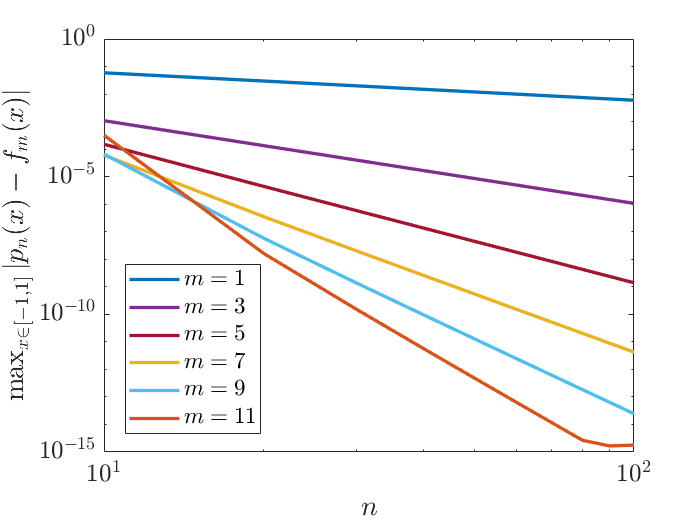
\includegraphics[scale=0.5]{graphics/plot-07-02.png}
    \caption{Infinity-norm error of $f(x) = |x|^m$ in $[-1, 1]$}
  \end{figure}
\end{solution}

\begin{statement}{c}
  Based on the result of parts (a) and (b), form a hypothesis about the asymptotic behaviour
  of the error for fixed $m$ as $n \to \infty$.
\end{statement}

\begin{solution}
  From the graph in part (b), for a fixed value of $m$, we can form a hypothesis that
  \[
    \ln \max_{x \in [-1, 1]} |f(x) - p(x)| = -\alpha \ln n + \beta
  \]
  with $\alpha > 0$ and $0 < \beta < 1$.
  The infinity-norm error of $f$ is
  \begin{align*}
    \max_{x \in [-1, 1]} |f(x) - p(x)| &= \exp(-\alpha \ln n + \beta)\\
    &= \exp(-\alpha \ln n) \exp(\beta)\\
    &= \exp(\beta) \, n^{-\alpha}.
  \end{align*}.
  
  The theorem in the book requires an analytic function, however, even though our function
  only has $m - 1$ derivatives, experimentally the method converges and
  the infinity-norm error is $\mathcal{O}(n^{-\alpha})$.
\end{solution}